
\documentclass[final]{beamer}

\usepackage[scale=1.24]{beamerposter} % Use the beamerposter package for laying out the poster

%\usetheme{confposter} % Use the confposter theme supplied with this template
%\usetheme[faculty=chemo]{fibeamer} % Uncomment to use Masaryk University's fibeamer theme instead.

%\setbeamercolor{block title}{fg=ngreen,bg=white} % Colors of the block titles
%\setbeamercolor{block body}{fg=black,bg=white} % Colors of the body of blocks
%\setbeamercolor{block alerted title}{fg=white,bg=dblue!70} % Colors of the highlighted block titles
%\setbeamercolor{block alerted body}{fg=black,bg=dblue!10} % Colors of the body of highlighted blocks
% Many more colors are available for use in beamerthemeconfposter.sty

%-----------------------------------------------------------
% Define the column widths and overall poster size
% To set effective sepwid, onecolwid and twocolwid values, first choose how many columns you want and how much separation you want between columns
% In this template, the separation width chosen is 0.024 of the paper width and a 4-column layout
% onecolwid should therefore be (1-(# of columns+1)*sepwid)/# of columns e.g. (1-(4+1)*0.024)/4 = 0.22
% Set twocolwid to be (2*onecolwid)+sepwid = 0.464
% Set threecolwid to be (3*onecolwid)+2*sepwid = 0.708

\newlength{\sepwid}
\newlength{\onecolwid}
\newlength{\twocolwid}
\newlength{\threecolwid}
\newlength{\specialcolwid}
\setlength{\specialcolwid}{0.28\paperwidth}
\setlength{\paperwidth}{46.8in} % A0 width: 46.8in
\setlength{\paperheight}{33.1in} % A0 height: 33.1in
\setlength{\sepwid}{0.024\paperwidth} % Separation width (white space) between columns
\setlength{\onecolwid}{0.21\paperwidth} % Width of one column
\setlength{\twocolwid}{0.451\paperwidth} % Width of two columns
\setlength{\threecolwid}{0.678\paperwidth} % Width of three columns
%\setlength{\topmargin}{-0.5in} % Reduce the top margin size
%-----------------------------------------------------------

\usepackage{graphicx}  % Required for including images

\usepackage{booktabs} % Top and bottom rules for tables

%----------------------------------------------------------------------------------------
%	TITLE SECTION 
%----------------------------------------------------------------------------------------

\usepackage{graphicx}  % Required for including images

\usepackage{booktabs} % Top and bottom rules for tables

\usepackage{here}

\usepackage[utf8]{inputenc}

\usepackage[ngerman]{babel}

\usepackage{xcolor}

\usepackage{listings}

\definecolor{ui-blue}{HTML}{1857c4}
\definecolor{ui-red}{HTML}{cc0012}
\definecolor{docker-green}{HTML}{37974c}
\definecolor{docker-red}{HTML}{cd5458}
\definecolor{docker-lb}{HTML}{4c87e1}
\definecolor{docker-pu}{HTML}{8c0285}


\setbeamercolor{block title}{fg=white,bg=ui-blue}
\setbeamercolor{block body}{fg=black,bg=}


\title{Docker CheatSheet} % Poster title

\author{Tobias Köhler, Niklas Nikisch} % Author(s)

\institute{Hochschule Mannheim, Fakultät für Informatik} % Institution(s)

%----------------------------------------------------------------------------------------

\begin{document}
\addtobeamertemplate{block end}{}{\vspace*{2ex}} % White space under blocks
\addtobeamertemplate{block example end}{}{\vspace*{2ex}} % White space under example blocks
\addtobeamertemplate{block alerted end}{}{\vspace*{2ex}} % White space under highlighted (alert) blocks

\setlength{\belowcaptionskip}{2ex} % White space under figures
\setlength\belowdisplayshortskip{2ex} % White space under equations
%\begin{darkframes} % Uncomment for dark theme, don't forget to \end{darkframes}
\begin{frame} % The whole poster is enclosed in one beamer frame

%==========================Begin Head===============================
  \begin{columns}
   \begin{column}{\linewidth}
    \vskip1cm
    \centering
    \usebeamercolor{title in headline}{\color{fg}\Huge{\textbf{\inserttitle}}\\[0.5ex]}
    \usebeamercolor{author in headline}{\color{fg}\Large{\insertauthor}\\[1ex]}
    \usebeamercolor{institute in headline}{\color{fg}\large{\insertinstitute}\\[1ex]}
    \vskip1cm
   \end{column}
   \vspace{1cm}
  \end{columns}
 \vspace{1cm}

%==========================End Head===============================
\begin{columns}[t] % The whole poster consists of three major columns, the second of which is split into two columns twice - the [t] option aligns each column's content to the top

\begin{column}{\sepwid}\end{column} % Empty spacer column

\begin{column}{\specialcolwid} % The first column

%----------------------------------------------------------------------------------------
%	OBJECTIVES
%----------------------------------------------------------------------------------------

\begin{block}{Build}

\par Baut ein Image aus einem Dockerfile im Momentanen Verzeichnis und \textit{tagged} es.

\par \textbf{docker build} \textcolor{docker-pu}{\textbf{-t}} \textcolor{docker-lb}{\textbf{appname .}}

\vspace{1cm}
\par Listet alle Docker Images auf.
\par \textbf{docker images}

\vspace{1cm}
\par Entfernt das angegeben Image.
\par \textbf{docker image rm} \textcolor{docker-lb}{\textbf{ImageId}}

\end{block}

\begin{block}{Ship}

\par Einloggen um auf die Registry der Dockerseite zuzugreifen.
\par \textbf{docker login}

\vspace{1cm}
\par Lädt das getaggte Image in die Registry hoch.
\par \textbf{docker push} \textcolor{docker-lb}{\textbf{username}}/repository:\textcolor{docker-lb}{\textbf{tag}}

\vspace{1cm}
\par Tagged das Image für späteres hochladen.
\par \textbf{docker tag } $<$\textcolor{docker-lb}{\textbf{image}}$>$ \textcolor{docker-lb}{\textbf{username}}/repository:\textcolor{docker-lb}{\textbf{tag}}

\vspace{1cm}
\par Zieht ein Image oder ein Repository aus der Registry.
\par \textbf{docker pull} \textcolor{docker-lb}{\textbf{appname}}

\vspace{1cm}
\par Suche in der Registry nach einem Image.
\par \textbf{docker search} \textcolor{docker-lb}{\textbf{name}}


\end{block}

\begin{block}{Others}

\par Listet alle laufenden Container auf.
\par \textbf{docker container ls}

\vspace{1cm}
\par Stoppt den angegebenen Container.
\par \par \textbf{docker container stop} \textcolor{docker-lb}{\textbf{ContainerID}}

\vspace{1cm}
\par Entfernt den angegebenen Container.
\par \par \textbf{docker container rm} \textcolor{docker-lb}{\textbf{ContainerID}}

\vspace{1cm}
\par Listet alle laufenden Services auf.
\par \par \textbf{docker service ls} \textcolor{docker-lb}{\textbf{ContainerID}}†

\end{block}

\end{column} % End of the first column

\begin{column}{\sepwid}\end{column} % Empty spacer column

\begin{column}{\specialcolwid} % Begin a column which is two columns wide (column 2)

\begin{block}{Run}

\par Mit \textbf{docker run} können Container anhand von Images erstellt und gestartet werden. Das angegebene Baseimage wird zuerst lokal gesucht. Findet es keins, sucht es auf dem Docker Hub.
\vspace{1cm}


\par \textbf{docker run} \textcolor{docker-pu}{} \textcolor{docker-lb}{\textbf{appname}}
\vspace{1cm}

\par Startet die App aus dem Repository:
\par \textbf{docker run} \textcolor{docker-pu}{} \textcolor{docker-lb}{\textbf{username/repository:tag}}
\vspace{1cm}

\par Options:
\begin{itemize}
\item \textbf{-d} -- Startet den Container Im Hintergrund
\item \textbf{-it} -- Startet den Container im interactive-Modus, sodass man auf dem Container arbeiten kann.
\item \textbf{-p $<$host\_port$>$:$<$container\_port$>$} -- Mappt einen Port vom Container auf das Hostsystem
\item \textbf{--expose} -- Öffnet einen oder mehrere Ports
\item \textbf{-P} -- Mappt alle offenen Ports vom Container auf zufällige Hostsystem-Ports.
\item \textbf{--name} -- Gibt dem Container einen Namen, der anstelle der ID für Befehle verwendet werden kann
\item \textbf{-v $<$Datei\_oder\_Ordner\_zum\_mounten$>[$\:$>$Ziel\_auf\_dem\_Container$>]$} -- Mountet den angegebenen Ordner vom Hostsystem auf den Container, sodass dieser auf Dateien zugreifen kann.
\item \textbf{-e $<$VARIABLEN\_NAME$>$ \ = $<$VARIABLEN\_WERT$>$} -- Definiert eine Umgebungsvariable für den Container.
\item \textbf{--link $<$container\_name$>[$:$<$name\_in\_new\_container$>]$} --  Linkt einen bestehenden Container in den neuen, sodass sich der Container mit dem anderen Verbinden kann.
\end{itemize}


\begin{center}
\vspace{2cm}
Docker Ecosystem
\end{center}
\begin{figure}
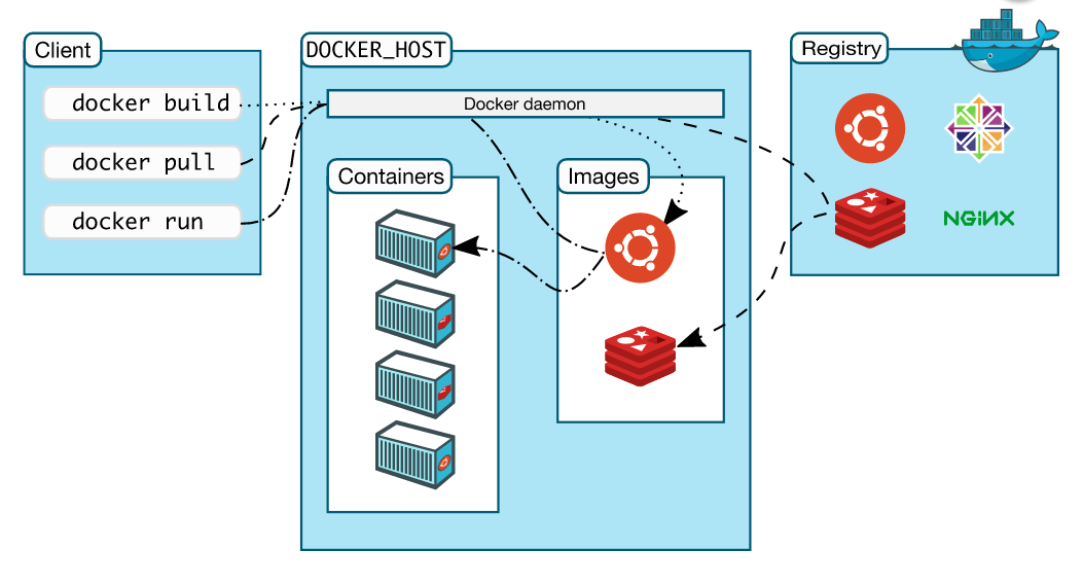
\includegraphics[scale=0.8]{eco}
\end{figure}

\end{block}



\end{column} % End of the second column

\begin{column}{\sepwid}\end{column} % Empty spacer column

\begin{column}{\onecolwid} % The third column




%----------------------------------------------------------------------------------------
%	CONCLUSION
%----------------------------------------------------------------------------------------

\begin{block}{Dockerfile}

\par \textcolor{docker-green}{\textbf{\# Nutzen eines Vaterimages}}
\par \textcolor{docker-pu}{\textbf{FROM}} \textcolor{docker-red}{\textbf{(Vaterimage)}}

\vspace{1cm}
\par \textcolor{docker-green}{\textbf{\# Setzt den Ordner in dem alle Befehle ausgeführt werden}}
\par \textcolor{docker-pu}{\textbf{WORKDIR}} \textcolor{docker-red}{\textbf{(Ordner)}}

\vspace{1cm}
\par \textcolor{docker-green}{\textbf{\# Kopiert Daten von (src) nach (des)}}
\par \textcolor{docker-pu}{\textbf{ADD}} \textcolor{docker-red}{\textbf{(url) (des)}}
\par \textcolor{docker-pu}{\textbf{COPY}} \textcolor{docker-red}{\textbf{(src) (des)}}

\vspace{1cm}
\par \textcolor{docker-green}{\textbf{\# Gibt einen Port frei}}
\par \textcolor{docker-pu}{\textbf{EXPOSE}} \textcolor{docker-red}{\textbf{(Nummer)}}

\vspace{1cm}
\par \textcolor{docker-green}{\textbf{\# Definiert ein Argument. Kann mit \$$<$ARG\_NAME$>$ darauf zugreifen.}}
\par \textcolor{docker-pu}{\textbf{ARG}} \textcolor{docker-red}{\textbf{(Argument)}}

\vspace{1cm}
\par \textcolor{docker-green}{\textbf{\# Definiert eine Umgebungsvariable}}
\par \textcolor{docker-pu}{\textbf{ENV}} \textcolor{docker-red}{\textbf{(Umgebungsvariable)}}

\vspace{1cm}
\par \textcolor{docker-green}{\textbf{\# Startet ein Programm mit übergebenen Parametern}}
\par \textcolor{docker-pu}{\textbf{CMD}} \textcolor{docker-red}{\textbf{["Programm", "Parameter"]}}

\vspace{1cm}
\par \textcolor{docker-green}{\textbf{\# Führt einen beliebigen Befehl auf dem Container aus}}
\par \textcolor{docker-pu}{\textbf{RUN}} \textcolor{docker-red}{\textbf{(Befehl)}}

\begin{small}
\vspace{1cm}
\par TIPP: Da bei jedem RUN ein neuer Container gecacht wird, kann man Befehle mit \&\& aneinander hängen um die Anzahl der Images/Layer zu reduzieren.

\vspace{1cm}
\par Bsp.: RUN apt-get update \&\& apt-get upgrade
	
\end{small}



\vspace{3cm}

\begin{figure}
\begin{minipage}[t]{0.40\textwidth}\vspace{0pt} 

\includegraphics[width=1.0\textwidth]{tobiaskohler} 
\begin{center}
	Tobias Köhler
\end{center}
\end{minipage}\hfill%
\begin{minipage}[t]{0.40\textwidth}\vspace{0pt} 
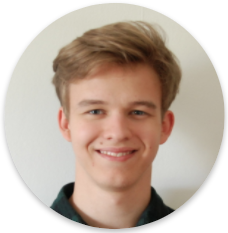
\includegraphics[width=1.0\textwidth]{niklasnikisch} 
\begin{center}
	Niklas Nikisch
\end{center}
\end{minipage}\hfill%

\end{figure}


\end{block}

%----------------------------------------------------------------------------------------

\end{column} % End of the third column

\begin{column}{\sepwid}\end{column} % Empty spacer column

\end{columns} % End of all the columns in the poster
\end{frame} % End of the enclosing frame
%\end{darkframes} % Uncomment for dark theme
\end{document}
